
% \clearemptydoublepage
% \setcounter{figure}{0}
% \setcounter{tableEng}{0}
% \setcounter{algocf}{0}
% \chapter{基于可微分渲染的纹理优化}

\chaptera{基于可微分渲染的纹理优化}

\section{引言}
得益于消费机RGB-D相机的普及,人们能够很容易的对真实世界的场景进行建模得到场景和物体的三维模型。近几年,基于RGB-D的三维重建方法取得了前所未有的进步。然而,纹理优化/重建的关注度不如几何重建高,对于游戏、混合现实、虚拟现实等娱乐化数字产业来说纹理细节往往比几何细节更加重要。最近的工作\upcite{RichardNewcombe2011KinectFusionRD,ThomasWhelan2012KintinuousSE,ThomasWhelan2015ElasticFusionDS,SungjoonChoi2015RobustRO,VictorAdrianPrisacariu2017InfiniTAMVA,niessner2013real}已经可以获取高质量几何模型,但是纹理获取结果的质量无法令人满意。\par

造成这一现象的直接原因在于重建模型本身的形状缺陷和相机位姿估计误差,导致纹理图像与几何模型发生错位或者纹理映射关系混乱,使得最终生成的纹理在视觉上会出现模糊伪影等现象。从本质上看,有以下几点因素使得纹理映射模型结果不尽人意。1)深度相机自身存在镜头误差和采集数据时受噪声影响使得计算深度距离时出现度量误差。2)重建算法中当前帧的相机位姿估计依赖于前一帧的相机位姿,某一帧相机位姿的估计误差会影响全局进而发生相机漂移或者追踪失败。3)采集的深度图序列和彩色图序列依靠时间戳来描述对应关系,二者相机快门不一定同步,产生错位现象。由于上述因素的影响,直接将多个视点图像投影到另一个与视角无关的纹理贴图的纹理映射过程中,不可避免地会产生模糊和重影伪影。所以,重建出的三维模型难以直接应用于其他领域,这是三维重建技术应用目前面临的难题。\par

由于消费级的深度相机拍摄的深度图分辨率较小、噪音大、视野小,测量距离有限。利用这样的深度数据进行重建不可避免的会出现几何细节的失真或丢失。在重建几何模型时,通常会使用TSDF技术来将多帧的深度数据融合到一个体素网格中。为了抵消重建过程中的噪声,每帧的TSDF值通常会采用加权平均策略进行融合,但这也会导致最终的重建模型失去一些锐利的几何细节。对于纹理映射,由于相机位姿估计误差及几何误差的存在,模型顶点投影至不同视角的彩色图像上,往往不会获得一致的颜色,在加权平均后顶点颜色会发生变化,最终生成的纹理在视觉上非常模糊。为了得到清晰的纹理,先前的工作使用不同的方法来克服重建模型中的误差。Zhou等人\upcite{zhou2014color}采用非刚性扭曲来抵抗相机位姿存在的误差。Bi等人\upcite{bi2017patch}采用基于块合成方法,重生成纹理图以补偿几何模型和相机位姿中的误差。Fu等人\upcite{fu2018texture}采用全局到局部优化方法以矫正投影矩阵以及纹理坐标。最近Huang等人\upcite{JingweiHuang2020AdversarialTO}借助对抗神经网络,学习误差容忍度量,并使用像素重生成管线重新合成新的纹理图像。虽然生成对抗网络有强大的生成能力,对多种不同误差都有很好的抵抗效果。但是当某些误差因素过大时,如相机位姿,重生成的纹理图像仍然存在模糊伪影现象。因此本文对相机位姿单独进行优化后再借助生成对抗网络重新生成具有照片级清晰度的纹理图像。\par
基于深度学习的方法在鲁棒性和易用性等方面相对于传统的纹理优化方面有优势,因为神经网络可以识别模型重建过程的各种噪声,然后重新生成新的适配与几何模型的纹理抵抗这些噪声。然而,随着误差值的上升,纹理图像的合成效果逐渐下降,尤其是在图像对应的相机位姿非常不准确的情况下。某些数据集上由于相机估计误差较大,几何模型顶点投影不同的彩色图像上,往往得到不同的颜色,在加权融合后纹理会非常模糊,而且单纯用对抗神经网络合成的纹理图无法根除这一现象。由Fu等人\upcite{fu2018texture}的工作得到启发,本文将优化算法和纹理合成算法有机地结合起来。首先,借助于梯度下降算法,更新每个视角对应的相机位姿。然后,对每个顶点投影至可见视角中获取的颜色做加权平均处理生成纹理。对于纹理中存在模糊区域,则借助对抗生成网络重新合成。\par
传统的相机位姿矫正算法往往借助李群和李代数\upcite{sola2018micro}理论矫正相机位姿,计算代价高。受可微分渲染在单视图三维重建\upcite{liu2020general}\upcite{ShichenLiu2019SoftRA}中的成功启发,借助于可微分渲染可以对三维场景的各个组件进行优化,如顶点位置、灯光、相机投影矩阵等。借助于梯度下降算法更新渲染器所含元素,并且很容易集成到神经网络中而无需额外参数。经过实验证明,优化相机后生成的纹理与初始的纹理相比模糊伪影区域显著减少,接近于真实场景的外观。经过对抗生成网络后可以恢复出模型真实表面外观。本文算法在公共数据集上的定量和定性结果表明,相对于仅使用优化法或合成法的纹理优化算法,本文算法在性能和效果方面均有显著提高。


\section{算法流程}
\begin{figure}[!t]
    \centering
    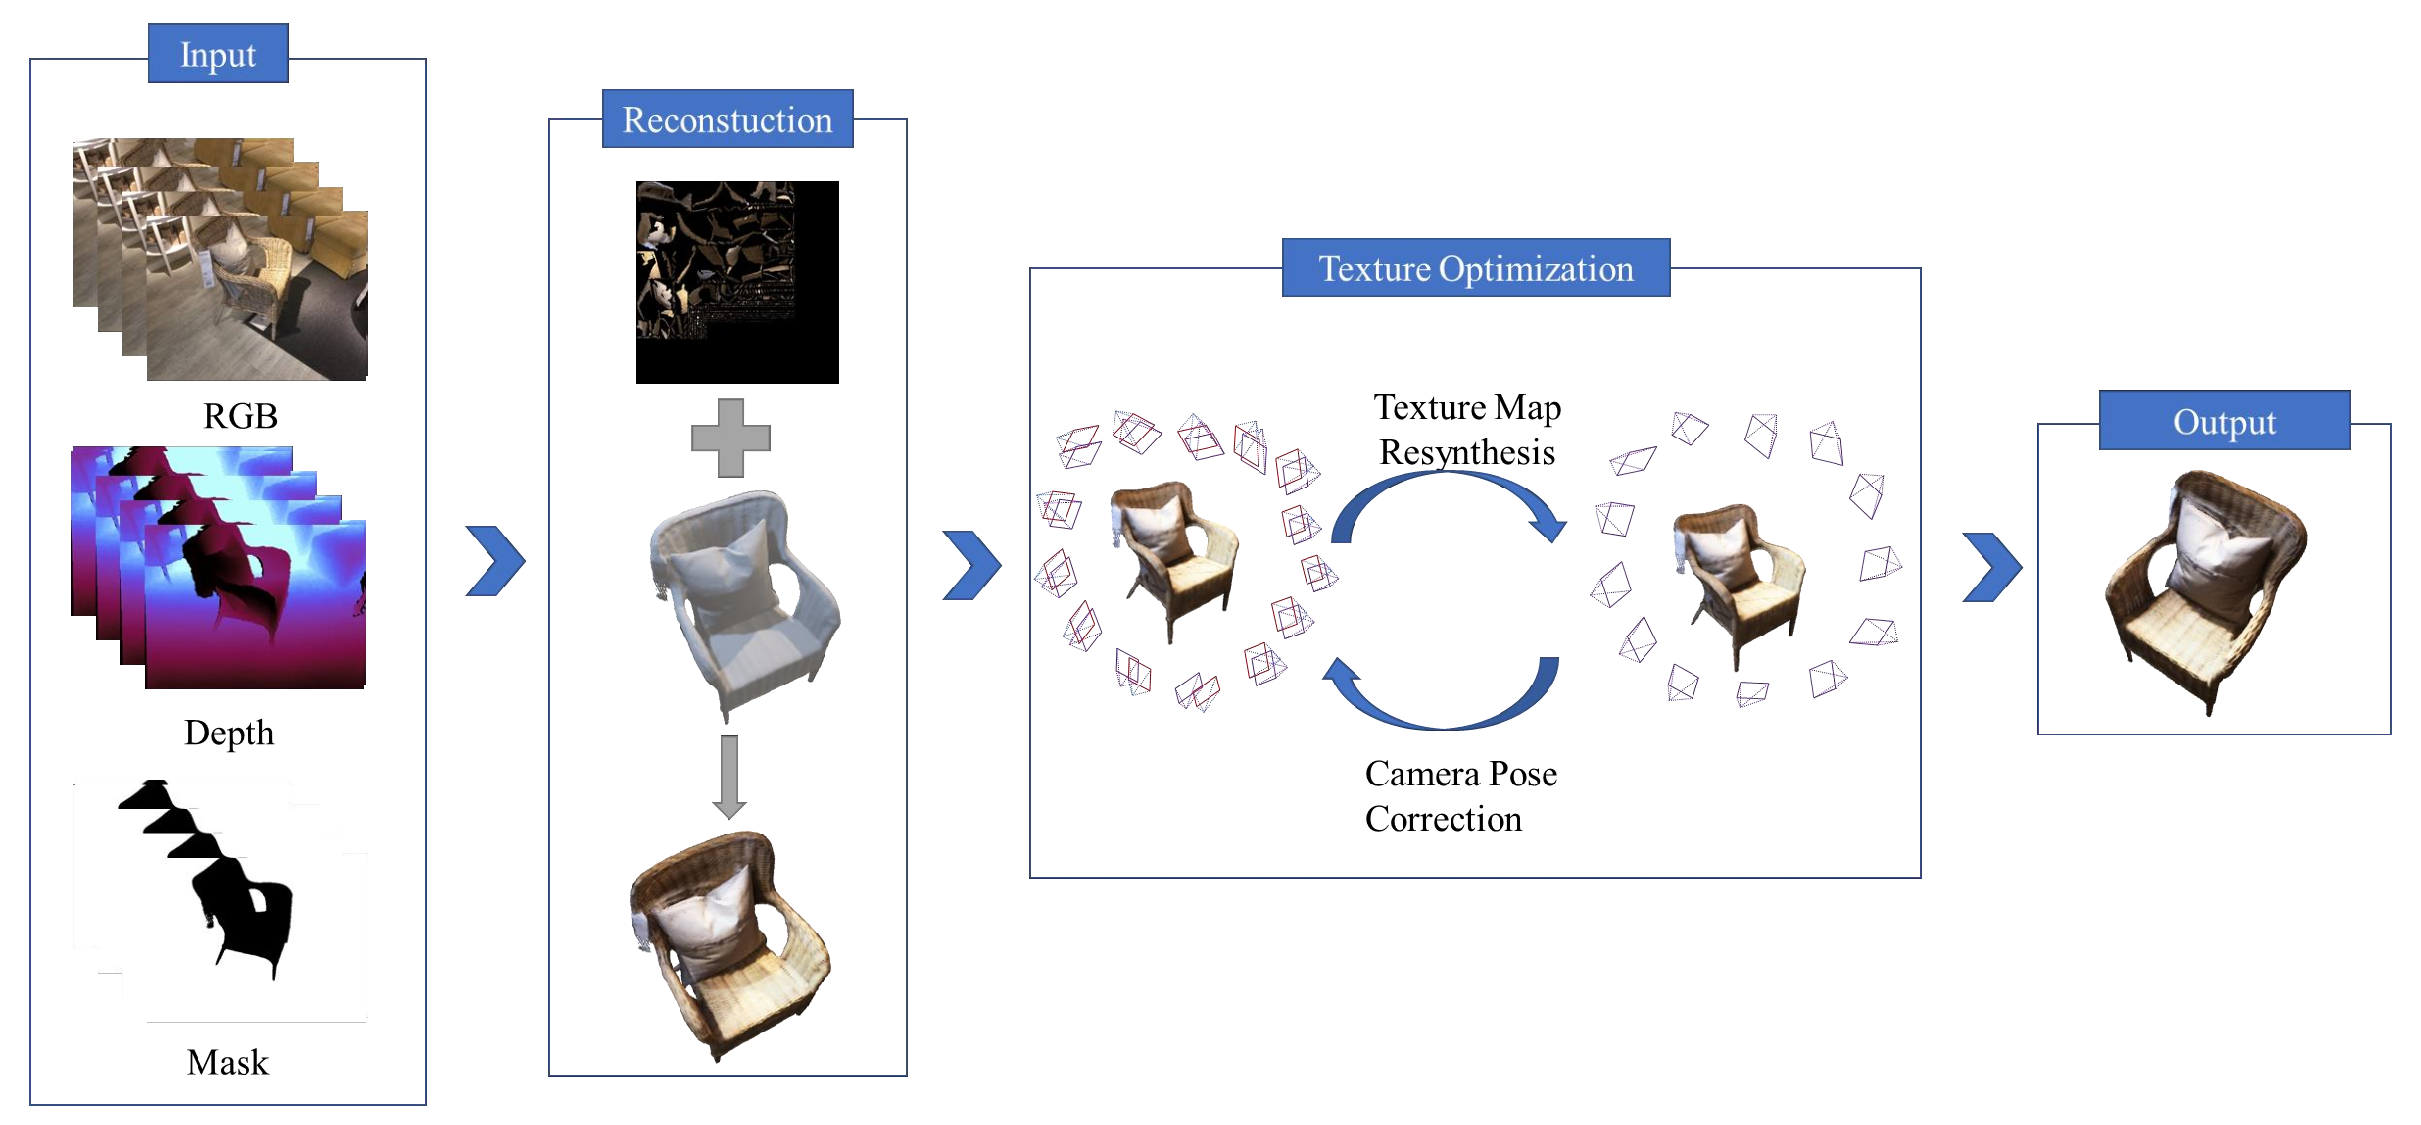
\includegraphics[width=1\columnwidth]{pic/work1/work1.pdf}
    \bicaption{基于可微分渲染的纹理优化概述}{The overview of texture optimization based on differentiable rendering}
    \label{fig:work1}
\end{figure}

本文旨在通过RGB-D相机采集的深度图片和彩色图片,并将不同视角的彩色图适配到几何模型上以生成具高保真的纹理贴图。为了达成这一目标,本文提出结合相机位姿矫正与纹理合成算法提高纹理模型的清晰度和保真度。如图~\ref{fig:work1}所示,算法以彩色图、深度图和相应的掩码图作为输入,通过三维重建得到初始的重建模型。在纹理优化阶段,首先利用可微分渲染矫正相机位姿,接着,利用对抗生成网络合成一幅新的纹理图像,以适配重建模型。具体地、本文的算法分为四个步骤。\par
\noindent\textbf{模型重建:}RGB-D相机采集的原始数据为图片或者视频格式,需要进一步处理转换为同步的的彩色图序列和深度图序列。在公共数据集上,一般会提供深度图集、彩色图集、对应的相机内外参以及用重建算法\upcite{SungjoonChoi2015RobustRO,AngelaDai2016BundleFusionRG,RichardNewcombe2011KinectFusionRD}重建出的初始几何模型。在极少数没有提供几何模型和相机位姿的数据集上,本文通过重建算法\upcite{LongYang2018SurfaceRV}重建初始的几何模型并估计初始的相机位姿。\par
\noindent\textbf{预处理:}在预处理阶段,本文从所有帧中选出最清晰的彩色图像当作候选图像,消除冗余和重叠度较高的视角的影响。同时确保所选关键帧所代表的视角覆盖范围与原始数据集一致。额外采用多视角进行监督,避免单视角因相机漂移导致位姿异常值影响纹理优化过程。具体地,本文为每一帧都选取邻近视角,训练时使用用源视角和扭曲后的视角共同监督。\par
\noindent\textbf{相机位姿矫正:}为了借用可微分渲染框架矫正相机位姿,首先渲染三维模型至某一视角的彩色图像,然后再将真实图像与渲染图像经过损失函数优化相机投影矩阵。矫正相机位姿完成后,再通过将模型的顶点投影至所有可见视角,并采用加权平均算法来融合对应颜色,生成纹理图像。为了便于后续纹理优化,本文将以UV纹理形式保存至二维图像中。\par
\noindent\textbf{纹理优化:}受图像翻译模型\upcite{isola2017image,wang2018high}的启发,本文借助对抗生成网络,以初始纹理为基础生成新的UV纹理。在获取纹理到图像的映射关系和相对准确的相机位姿后,再用源视角$I_A$的邻近视角$I_B$扭曲到源视角当作真例,渲染图像为假例,用对抗生成模型优化纹理图。\par

\subsection{数据预处理}
\noindent\textbf{重建模型:}对于RGB-D数据集,本文使用消费级深度相机kinect \emph{v}1或者kinect \emph{v}2在固定曝光和白平衡模式下拍摄。拍摄完成后,可以得到深度图集和彩色图集以及相机标定后的内参,并没有相机位姿与重建模型。由最近的纹理优化方法G2Tex\upcite{fu2018texture}得到启发,本文也借鉴G2Tex模型重建方案。其初始输入为深度相机扫描的深度图集合和彩色图集合,并借助基于RGB-D三维重建算法\upcite{LongYang2018SurfaceRV}利用稀疏序列融合(Sparse-Sequence Fusion,SSF)的增强策略,获取高可用、高质量的RGB-D序列重建TSDF模型,最后使用移动立方体算法提取出网格模型。重建几何模型的关键帧选取策略依照如下公式进行:
\begin{equation}
E(i)= \lambda_{1} E_{\mathrm{jit}}(i)+\lambda_{2} E_{\mathrm{dif}}(i)+\lambda_{3} E_{\mathrm{vel}}(i)+\lambda_{4}E_{\mathrm{cla}}(i)+E_{\mathrm{sel}}(i)
\end{equation}
其中,$E_{\mathrm{sel}}(i)$表示当前帧$i$是否作为三维重建的有效帧的控制项,$E_{\mathrm{jit}}(i)$用于度量当前帧$i$与上一个有效帧的抖动强度比较,尽量保证选取平滑非抖动帧进行重建,$E_{\mathrm{dif}}(i)$确保前后有效帧间有超过阈值重叠覆盖率,避免相机跟踪失败,$E_{\mathrm{vel}}(i)$度量相机运动速度,避免相机运动过快产生的模糊帧,$E_{\mathrm{cla}}(i)$是图像清晰度度量指标,衡量彩色图片清晰度以保证选择的彩色图像最清晰。经过重建算法后本文得到初始网格模型$M$。\par
\noindent\textbf{关键帧获取。}由于RGB-D相机是手持进行拍摄,拍摄过程中不可避免出现相机抖动或者相机镜头平移速度过快的情况,使得拍摄的图片出现内容模糊、失真等现象。为了根除这个现象,本文会根据 Crete 等人 \upcite{FrederiqueCrete2007TheBE}提出的图片的模糊度度量指标评估每一个彩色帧。对于彩色图超过100张的数据集,本文设置一个大小为5的滑动窗口,在每个窗口内选择模糊度最小的图片作为关键帧$KF$,根据数据集的大小灵活调整窗口大小。经过实验证明选择关键帧并不仅不会影响优化效果而且会线性减少优化时间。 \par
\noindent\textbf{辅助视角选取。}受Huang等人\upcite{JingweiHuang2020AdversarialTO}的启发,本文为每个原始视角$T_s$选取一个辅助视角$T_t$,使得辅助视角重投影至原视角作为真例以此来监督渲染的图片。令$p_s$,$p_t$分别表示原始视角和目标视角的齐次坐标,则二者的对应关系可以描述为:
\begin{equation}
	p_s\sim KT_{t\rightarrow s}D_tK^{-1}p_t \label{work1:wrap}
\end{equation}
其中,$D_t$表示目标视角的深度值。由于遮挡和深度图存在噪声的缘故,目标视口扭曲到原始视角因未对齐会产生残缺现象。为了防止残缺部分过大,本文计算任意两个视口计算z方向夹角$\theta$,当$\theta\le15^{\circ}$时,两个视角加入至源视角-目标视角位姿集合。

\subsection{相机位姿矫正}
\begin{figure}[ht]
    \centering
    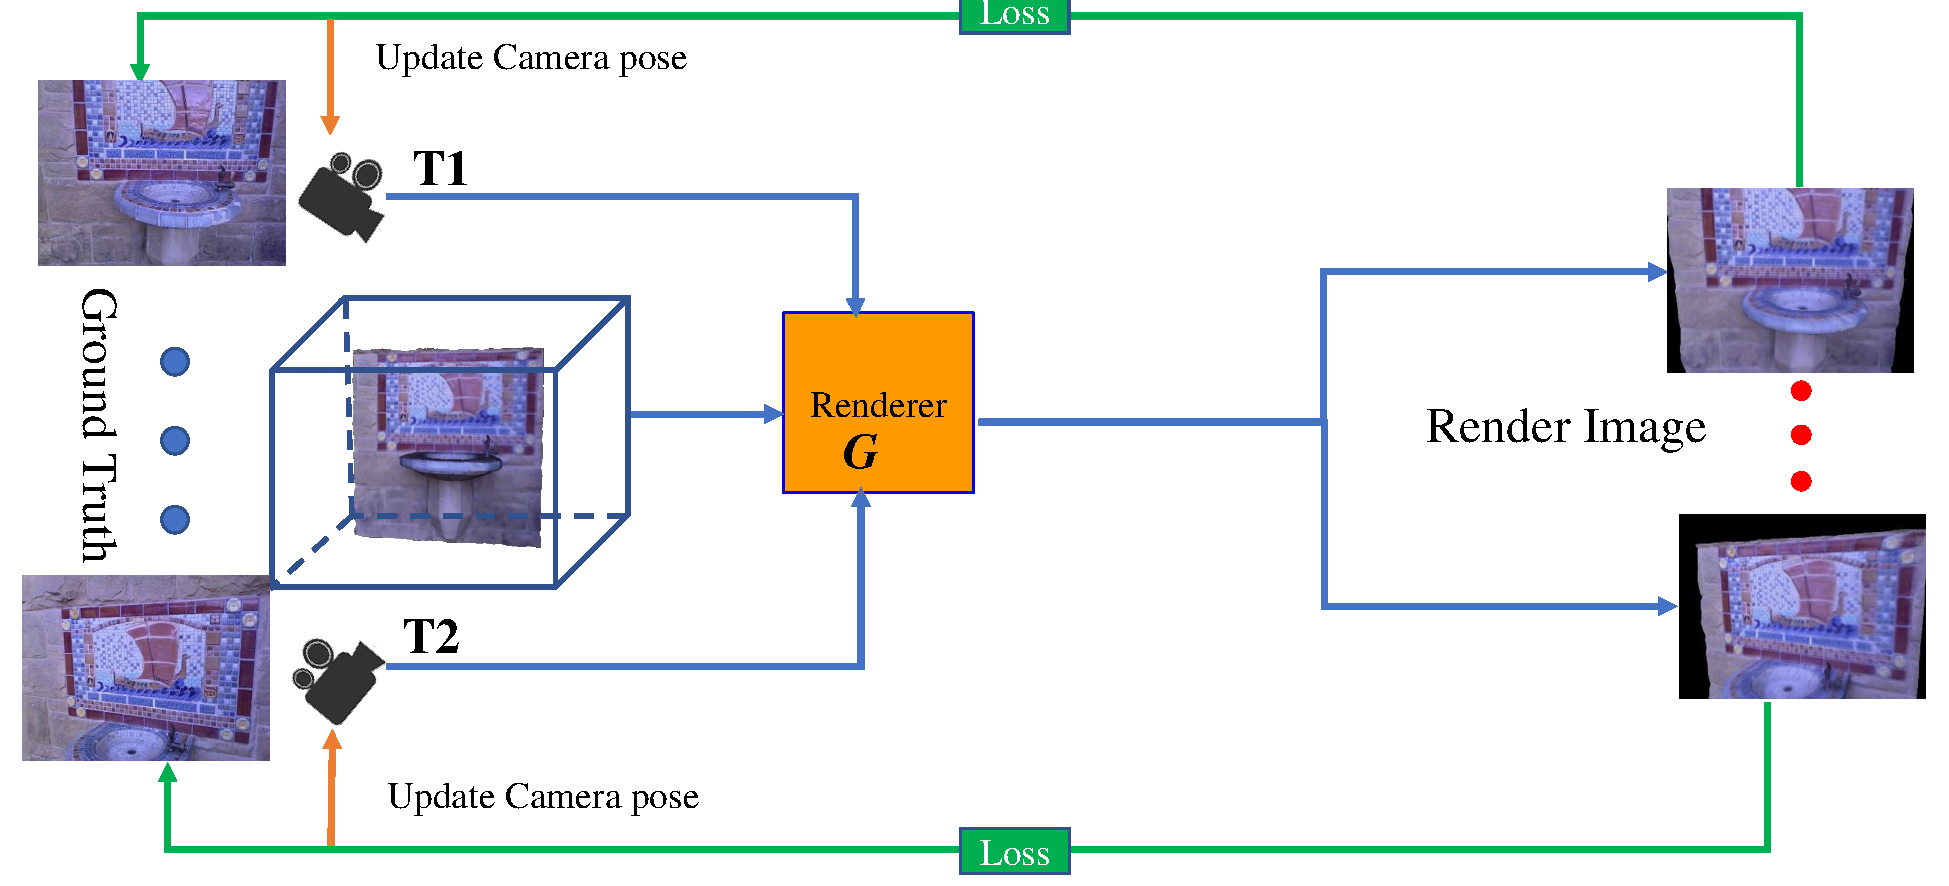
\includegraphics[width=1\columnwidth]{pic/work1/cameras.pdf}
    \bicaption{基于可微分渲染的相机位姿矫正概述}{Overview of camera pose correction based on differentiable Rendering}
    \label{fig:cameras}
\end{figure}

在本节中,本文会详细介绍相机位姿矫正的原理与步骤。如图~\ref{fig:cameras}所示,本文算法的核心在于利用渲染技术渲染模型至不同视角,然后再利用光度一致性误差,产生梯度更新相机位姿矩阵。在模型渲染中,模型会进行刚体变换和透视投影操作。刚体变换的旋转表示有旋转矩阵、欧拉角、轴角表示、四元数等。本文采用旋转矩阵表示,一方面易于向其它表示方式转换,另一方面易于将顶点位置变换到笛卡尔坐标系下。令$ \left \{ \mathbf{I_i} \right \} $表示输入图像集合,$\left \{ \mathbf{T_i} \right \}$表示相机位姿集合,$\left \{ \mathbf{P_i} \right \}$表示图像对应的模型顶点集合。旋转矩阵定义为:
\begin{equation}
	T = \left[\begin{array}{cc}
		R & t \\
		0 & 1
	\end{array}\right]
\end{equation}
$T \in \mathbf{SE}(3)$,$R \in \mathbf{SO}(3)$并且$t\in\mathbb{R}^3$,其中,$T \in \left \{ \mathbf{T_i} \right \}$为4$\times$4矩阵。\par 
将三维重建模型定义在世界坐标系下,并以模型中心为坐标原点。经过刚体变换后,以相机所在位置为坐标原点,模型位于相机正前方。然后,本文采用透视变换将处于相机坐标系下的模型顶点投影至二维图像平面上。根据相机成像模型定义刚性变换为$\mathbf{G}(p)=Tp$,$p \in \left \{ \mathbf{P_i} \right \}$,变换后的顶点齐次坐标为$\mathbf{g}=[g_x, g_y, g_z,g_w]^\top$。设投影图像平面变换为$\mathbf{U}$,本文按照以下公式计算图像平面中的像素位置:
\begin{equation}
\mathbf{U}\left(g_{x}, g_{y}, g_{z}, g_{w}\right)=\left(\frac{g_{x} f_{x}}{g_{z}}+c_{x}, \frac{g_{y} f_{y}}{g_{z}}+c_{y}\right)^{\top} \label{project}
\end{equation}
其中,$f_x,f_y$表示相机在$x,y$方向的焦距长度,$c_x,c_y$分别表示光轴对于投影平面坐标中心的偏移量。这些参数可以利用相机标定获取\upcite{888718}。\par


在基于RGB-D的三维重建中常使用基于三维点云配准的最近邻迭代(Iterative Closest Point,ICP)\upcite{besl1992method,chen1992object}及其衍生算法估计初始的相机位姿。由于存在噪声相机位姿估计存在累积误差,即使后续优化中采用回环检测矫正,也并不能完全消除存在的误差。使用不完美的相机位姿渲染图片,渲染图片和采集图片会发生错位现象。在传统的优化相机方案中,通常计算网格顶点重投影误差来优化相机投影矩阵$T$。设模型上一顶点$p$,初始颜色为$C(p)$(初始颜色,利用顶点投影后的像素颜色平均可得),定义$\Gamma(x,y) $为灰度图像上$(x,y)$位置的颜色值。顶点颜色与投影至视角$i$上的像素颜色值会存在差值,定义残差项为:
\begin{equation}
	R_{i, \mathbf{p}}=C(\mathbf{p})-\Gamma_{i}\left(\mathbf{U}\left(\mathbf{G}\left(\mathbf{p}, \mathbf{T}_{i}\right)\right)\right)
\end{equation} \par
定义优化目标为:
\begin{equation}
	E(\mathbf{T})=\sum_{i} \sum_{\mathbf{p} \in \mathbf{P}_{i}} R_{i, \mathbf{p}}^{2}
\end{equation}

利用高斯牛顿迭代算法\upcite{wedderburn1974quasi}对上述公式进行迭代求解,并且更新一次相机位姿$T$后,重新计算每个顶点的颜色$C(p)$,最终获得精确的相机位姿以及帧间一致的顶点颜色。受传统优化方法得到启发,本文借助于可微分渲染算法投影顶点至图像平面,使用UV纹理保存顶点颜色,通过$L_1$范数度量图像间的颜色差异,最后用梯度下降算法优化相机位姿矩阵$T$。\par
考虑到渲染能力和效率,以及本文无需对模型表面材质进行额外建模,因此使用基于SoftRas的渲染框架\upcite{ravi2020pytorch3d}和布林冯着色模型\upcite{blinn1977models},渲染目标遵从以下规则:
\begin{equation}
	C_i = (I_a + I_d) * P_i + I_s
\end{equation}
其中,$I_a$,$I_d$,$I_s$分别表示环境光系数、漫反射光和高光系数。$C_i$,$P_i$分别表示彩色图像素和纹理像素。为了最大限度的还原具有高保真度的纹理,本文只保留环境光,设置高光和漫反射光系数为0。对于相机外参$T$,本文采用以上介绍的投影和表示方法。渲染框架的所有模块都是可微分的,而且不会增加参数量,因此可以直接作为神经网络的一部分,进行端到端的训练。具体地,每一次渲染本文会随机选择某个视角,在该视角下生成彩色图$\tilde{I}_c$深度图$\tilde{I}_d$以及轮廓图$\tilde{I}_s$,即$\tilde{I}_c,\tilde{I}_d,\tilde{I}_s = Render(M_0|T_i)$。令$I_c, I_d, I_s$分别表示彩色图、深度图和掩码图真值。本文首先使用光度一致性损失来优化已选帧的相机位姿。
\begin{equation}
	E_c = \left \| I_c - \tilde{I}_c  \right \|_1 
\end{equation}

然而,仅仅具有光度一致性损失不足以约束相机位姿以朝着本文期望的方向更新,在某些场景中纹理较为单一或者纹理细节较少时,仍有可能发生相机漂移现象。因此,本文额外考虑深度图损失,以增加几何一致性的约束。
\begin{equation}
	E_d = \left \| I_d - \tilde{I}_d  \right \|_1 
\end{equation}

受SoftRas\upcite{ShichenLiu2019SoftRA}启发,本文也采用轮廓损失来对几何进行约束。这个轮廓损失函数为:
\begin{equation}
	E_s = 1 - \frac{\left \| \hat{I_s}\otimes I_s  \right \|_1 }{\left \| \hat{I_s}\oplus  I_s- \hat{I_s}\otimes I_s \right \| }_1  
\end{equation}
其中,$\otimes $和$\oplus $分别是按元素计算的乘法运算符和求和运算符。最后本文按照各个损失对优化相机参数的贡献来赋予每个损失不同的权重系数。在实验研究中,本文设置权重系数为$\lambda_c = 0.1$,$\lambda_d = 1$,$\lambda_s = 1$。\
\begin{equation}
	L_T = \lambda_c E_c + \lambda_d E_d +\lambda_s E_s \label{pose}
\end{equation} \par

需要注意的是,在不同的场景下,本文可能需要微调优化相关的超参数,而且相机位姿本身没有真实值可供参考。因此,评估相机位姿的准确性唯一的方法是使用矫正后的相机位姿$T'$生成新的纹理图像,并将其与原始纹理进行比较。若新生成的纹理图像越清晰,则说明优化的效果越好。


\subsection{纹理重合成}

\begin{figure}[ht]
    \centering
    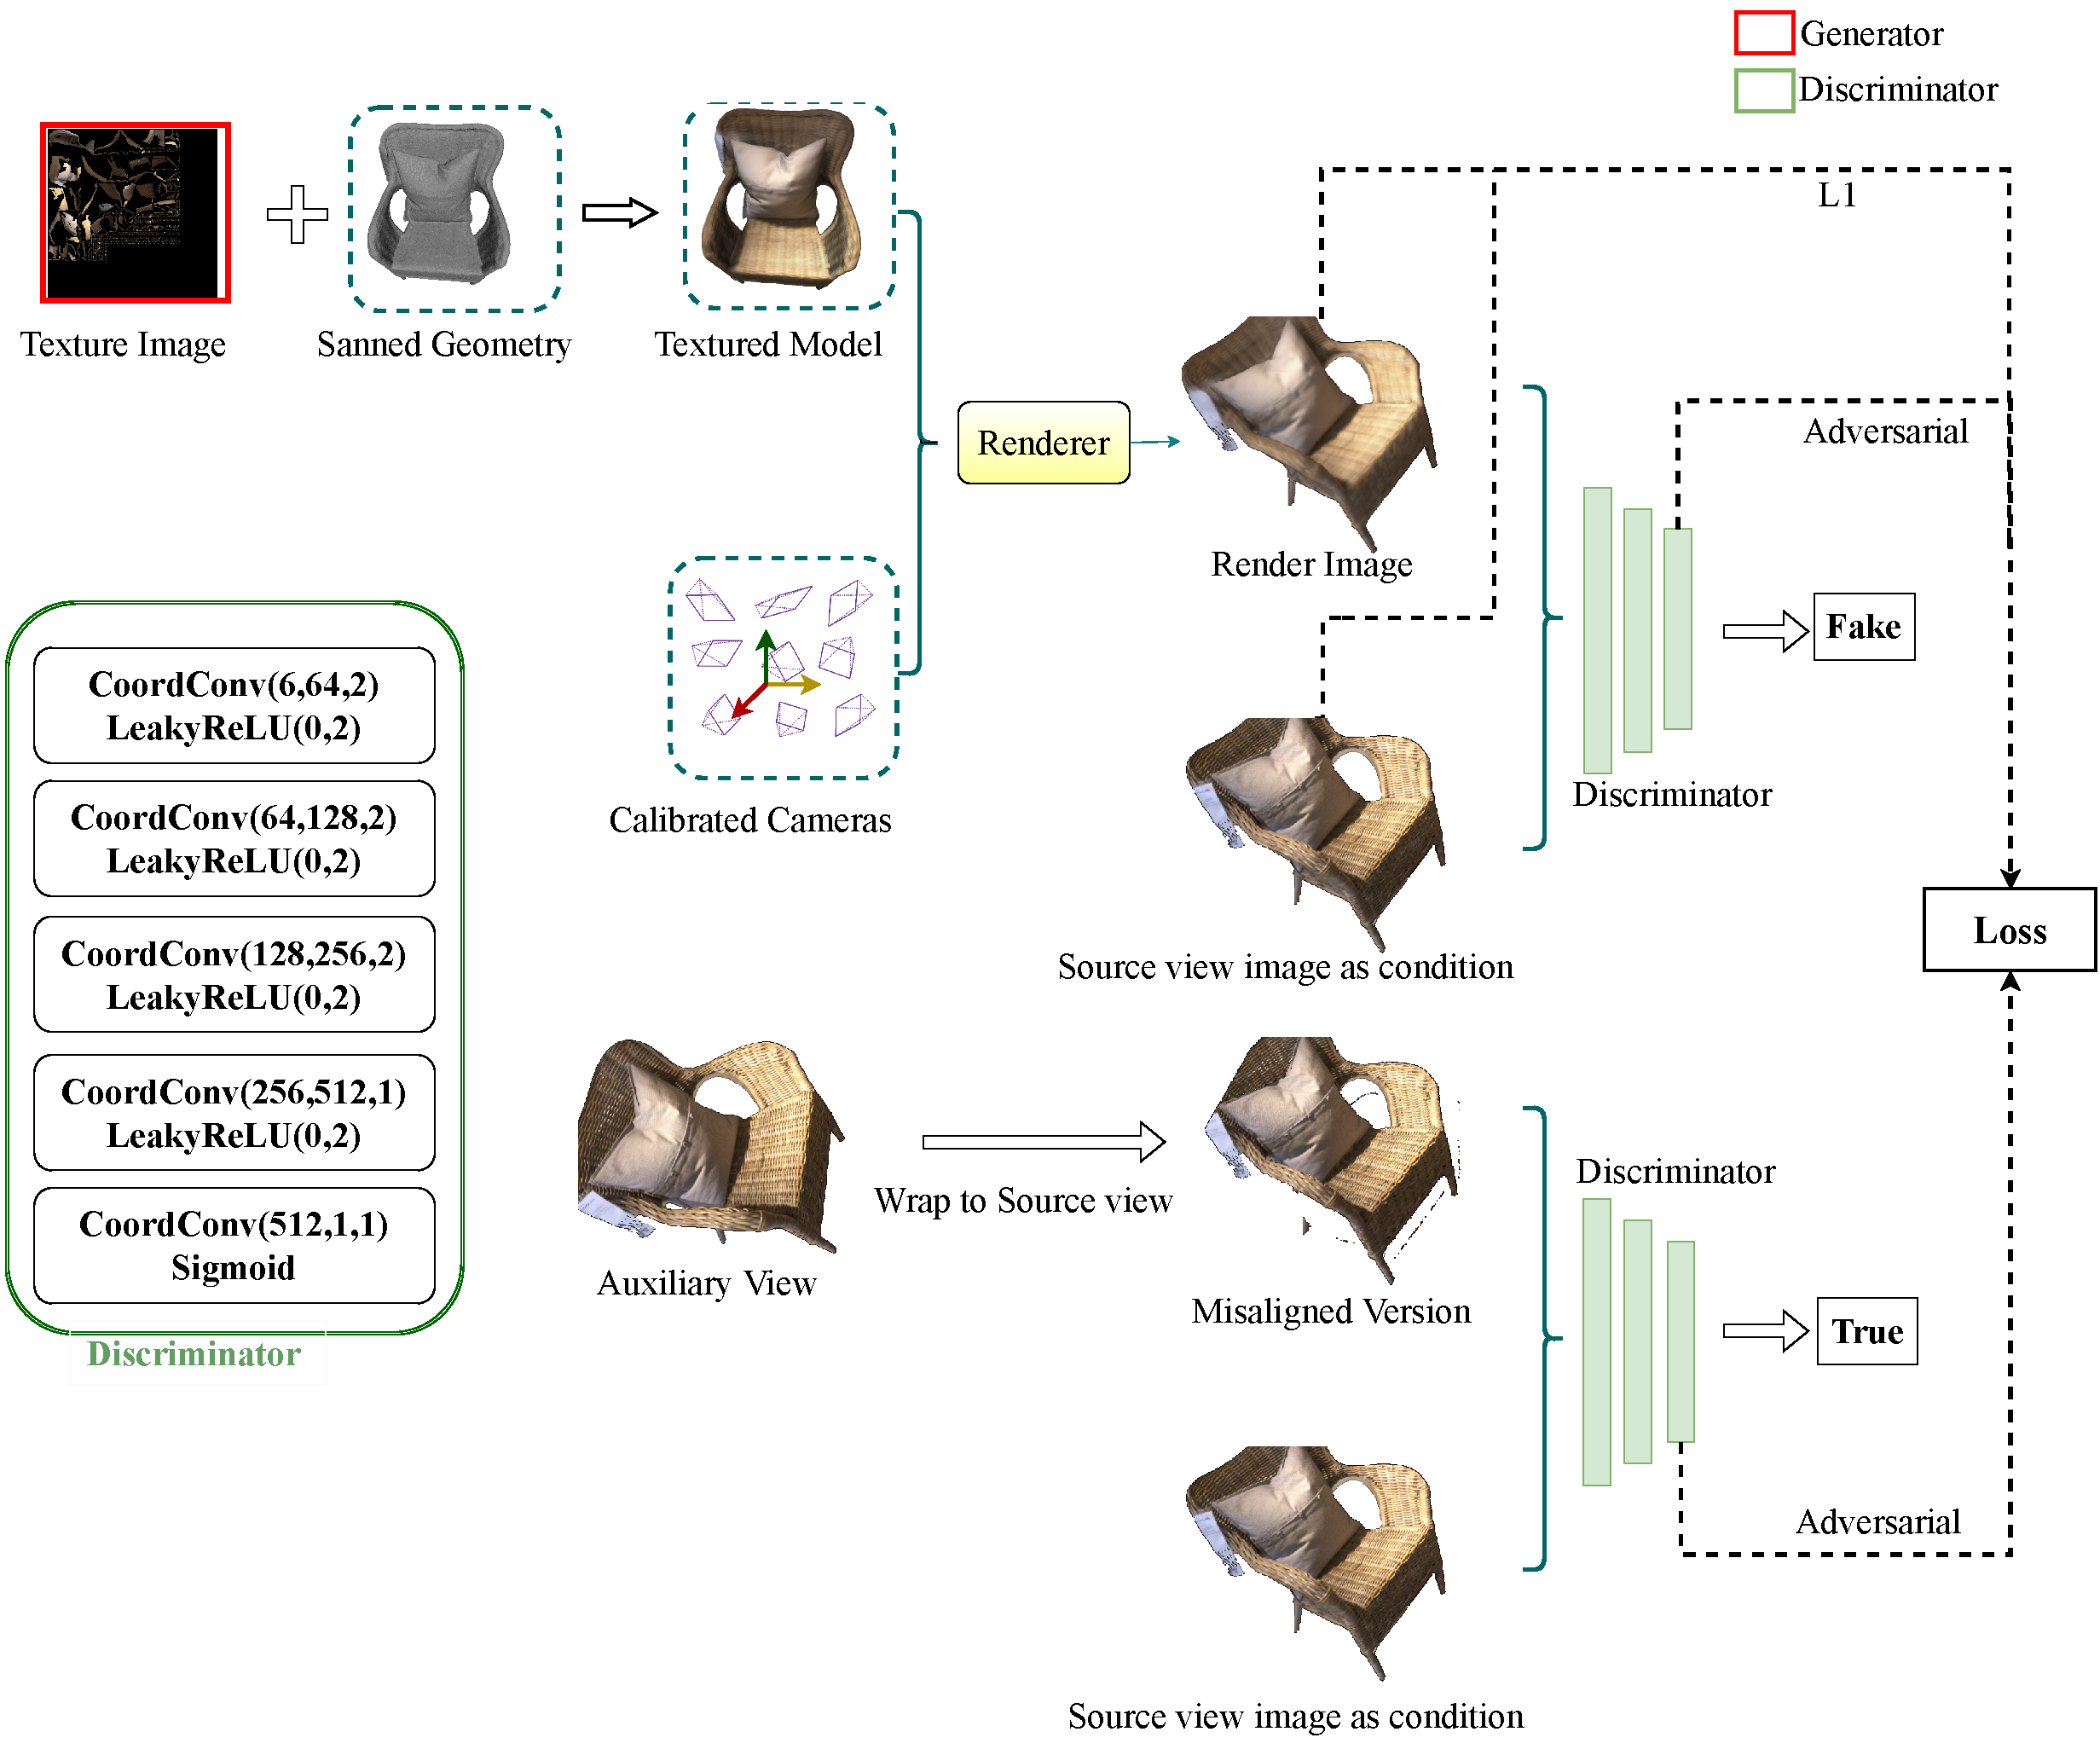
\includegraphics[width=1\columnwidth]{pic/work1/Texture.pdf}

    \bicaption{基于GAN的纹理图像优化概述}{Overview of texture image optimization based on GAN}
    \label{fig:Texture}
\end{figure}

仅仅矫正相机位姿是不够的,优化结果并不能完全消除噪声。传统方法中单纯优化相机步骤后,结果往往需要结合网格细分或者扭曲纹理图像或者纹理坐标,使得进一步使得图像与几何模型对齐,从而抵抗重建模型的噪声以弥补几何误差带来的影响。对于本文的纹理优化算法,本质上也存在这个问题。况且,本文采用顶点加权融合方式生成的纹理,在局部区域会存在模糊并且会丢失细节现象。受到Huang等人\upcite{JingweiHuang2020AdversarialTO}的启发,本文使用对抗生成网络来学习重建模型和拍摄的彩色图片之间错位的容忍度。本文使用基于$\pi$GAN\upcite{chanmonteiro2020pi-GAN,liu2018intriguing}的判别器,通过像素重生成管线合成纹理图。网络结构类似于pix2pix\upcite{isola2017image}的条件对抗网络,利用判别器$D$学习区分真实图片和渲染图片,并产生多视角一致性的纹理图像。本文使用辅助视角重投影至原视角$\boldsymbol{I}_{B \rightarrow A}$为真例,监督可微分渲染生成的彩色图像为假例,以更新纹理图像,并将原始视角的彩色图像作为生成对抗网络的条件。相应地,对抗损失函数定义如下:
\begin{equation}
	L_{a d v}=\log D\left(\boldsymbol{I}_{A}, \boldsymbol{I}_{B \rightarrow A}\right)+\log \left(1-D\left(\boldsymbol{I}_{A},\boldsymbol{I}_{A}^{D R}\right)\right) 
\end{equation}
其中,$\boldsymbol{I}_{A}^{DR}$表示基于源视角的渲染图像。为了使得对抗生成纹理的优化更加稳定,本文额外增加L1损失,避免优化过程陷入局部最小值,并提供初始的指导。L1损失定义如下:
\begin{equation}
L_T = \left \| \boldsymbol{I}_{A}- \boldsymbol{I}_{A}^{D R} \right \| 
\end{equation} \par
 最终本文的优化目标为:
\begin{equation}
	L = L_{adv} + \lambda L_T \label{texture}
\end{equation}

在优化期间,本文设置纹理图像$P$背景像素值为0,$\lambda$为10。每隔1000轮次会指数衰减$\lambda$的数值。\par
具体地,如图~\ref{fig:Texture}所示,对于每一次优化迭代,本文随机选择两个输入图像,$I_A$(源图像,图中所示Source view)和$I_B$(辅助图像,图中所示Auxiliary View),以及对应的相机姿态$T_A$和$T_B$,$I_A$作为GAN网络的条件。“真实图像”为按照公式\ref{work1:wrap}将辅助视角扭曲到源视角后得到图像$I_{B\to A}$(图中所示Misaligned Version)。由于遮挡和相机位姿不准确等因素,$I_{B\to A}$图像会发生残缺现象或者未残缺的部分与源图像$I_A$相比,像素会发生轻微的移位。“伪”图像是根据当前的相机位姿$T_A$从三维纹理模型渲染形成的图像(图中所示Render Image)。纹理的模糊伪影会反映至渲染图像上,判别器识别伪图像和真实图像间的差异,生成器重新生成纹理像素使得渲染图像和扭曲图像充分接近以匹配图像视角与纹理模型的映射关系。在纹理优化过程中,本文通过调整纹理像素的颜色,最大化生成损失,使得纹理图像在判别器视角下看起来更逼真。在判别器优化过程中,本文最小化对抗性损失,降低假样本与真样本之间的概率分布差异。最后,本文对总损失与L1损失函数进行线性组合,提高纹理优化效果。\par
经过若干次迭代交替训练判别器$D$和纹理$P$后,判别器会正确识别渲染图片中存在的伪影模糊或者裂缝现象,纹理图像会被重新生成,以弥补渲染图片和真实图片之间错位,使两者充分接近,达到欺骗判别器的目的。经过优化后的纹理相比与用加权融合方法生成的纹理更加真实,更接近于真实拍摄的彩色图片。\par


\subsection{迭代优化}

本文并未将优化方法和合成方法集成到一个模型中。相反,本文采用交替优化方案,以寻找生成最佳纹理。一般来说,矫正相机位姿和对抗生成网络合成纹理顺序可以交换,但是本文实验研究发现,先矫正相机姿态有助于提高纹理的保真度。一方面,相机位姿是纹理映射的核心,若相机位姿完全无误差,则不同视角直接贴在几何模型中就可以生成完美的纹理图。换句话说,位姿对纹理生成的影响最大。另一方面,合成纹理图也依赖于位姿变换,位姿越准确,合成效果越好。在外部迭代中,本文矫正相机位姿后再合成纹理模型,并且整个优化过程重复$N$次。在内部迭代中,本文根据不同场景设置相机位姿迭代次数$S_1$,纹理优化迭代次数$S_2$。一般情况下,本文设置$N \le 3,S_1 \le 40,S_2 \le 4000$,即可生成清晰的纹理图像。

\section{实验结果与讨论}
\paragraph*{\textbf{比较方法}}
在这个部分,本文会在公开的RGB-D数据集上,通过和以合成法为代表的纹理优化方法ATO\upcite{JingweiHuang2020AdversarialTO},以及以优化法为代表的纹理优化方法Zhou\upcite{zhou2014color},并使用他们在GitHub提供的源代码进行比较。由于Zhou采用顶点颜色加权融合方法生成纹理映射结果,最终结果以顶点颜色存储。这与本文和ATO使用UV纹理的纹理表示方案不同,其生成纹理的清晰度与顶点数目成正相关。为了公平起见,本文按照Zhou的选帧策略,选取最清晰的帧作为关键帧,并使用三角形中点细分方法对重建模型细分两次,以增加顶点数目。最后,设置优化轮次为关键帧数目的10倍。其它超参数均按照源代码给定的设置。本文在不同数据集的多个场景中进行了定性及定量实验分析,证明了本文方法的有效性。数据集既包含小场景,也包含大场景,既包含了含有丰富纹理细节的场景,也包含了单一纹理及弱纹理的场景。最后,本文将展示消融研究结果,以证明本文优化方案中各个组件的必要性。\par
% \paragraph*{\textbf{评估指标}}
\noindent\textbf{评估指标}\quad
为了对所生成的纹理进行定量研究,本文采用多种指标来衡量生成纹理与真实图片之间的差异。目前,纹理优化结果并没有一种行之有效的定量评估指标。一方面,因为大部分纹理映射算法会采用wrap图像的方法以适配几何模型,导致渲染图像无法完全与采集图像对齐。仅使用图像间的评估指标有待商榷。另一方面,纹理映射结果的表示形式多样,没有一个通用的标准形式。因此,评估纹理映射的好坏主要以\textbf{定性}比较为主。但是,定量评估指标能够在一定程度上反映纹理图像的清晰度和保真度。本文使用经典的图像间评估指标来进行定量分析,如峰值信噪比(Peak Signal-to-Noise Ratio,PNSR)\upcite{de2003improved}用于量化受损压缩影响的图像,能够反映图像的保真度,结果越高代表重建图像质量越好;结构相似性指数(Structural Similarity Index,SSIM)\upcite{brunet2011mathematical}是一种评价两张图片相似度的指标,它综合考虑了图片的亮度、对比度和结构信息,符合人类对图像的视觉感受,评价结果越高越好;学习感知图像块相似度(Learned Perceptual Image Patch Similarity,LPIPS)\upcite{zhang2018unreasonable}也称为感知损失,以神经网络计算误差的方法度量两张图像之间的差别,更符合人类的感知,其结果越小越好。在定量评估方面,首先渲染纹理模型至不同视角,并使用所有视角的结果的平均值来作为最终结果。


%\paragraph*{\textbf{训练设置}}
\noindent\textbf{训练设置}\quad
本章方法使用Ubuntu 18.04 LTS进行训练和测试,显卡为单个NVIDIA GeForce RTX3090 24GB,在训练网络时使用Adam优化器训练模型,并设置超参数$\beta_1=0.5,\beta_2=0.999,\epsilon =10^{-8}$。在矫正相机位姿时设置初始学习率为0.0001,用对抗生成优化纹理时设置初始学习率为0.01。


\begin{figure}[!t]
\centering
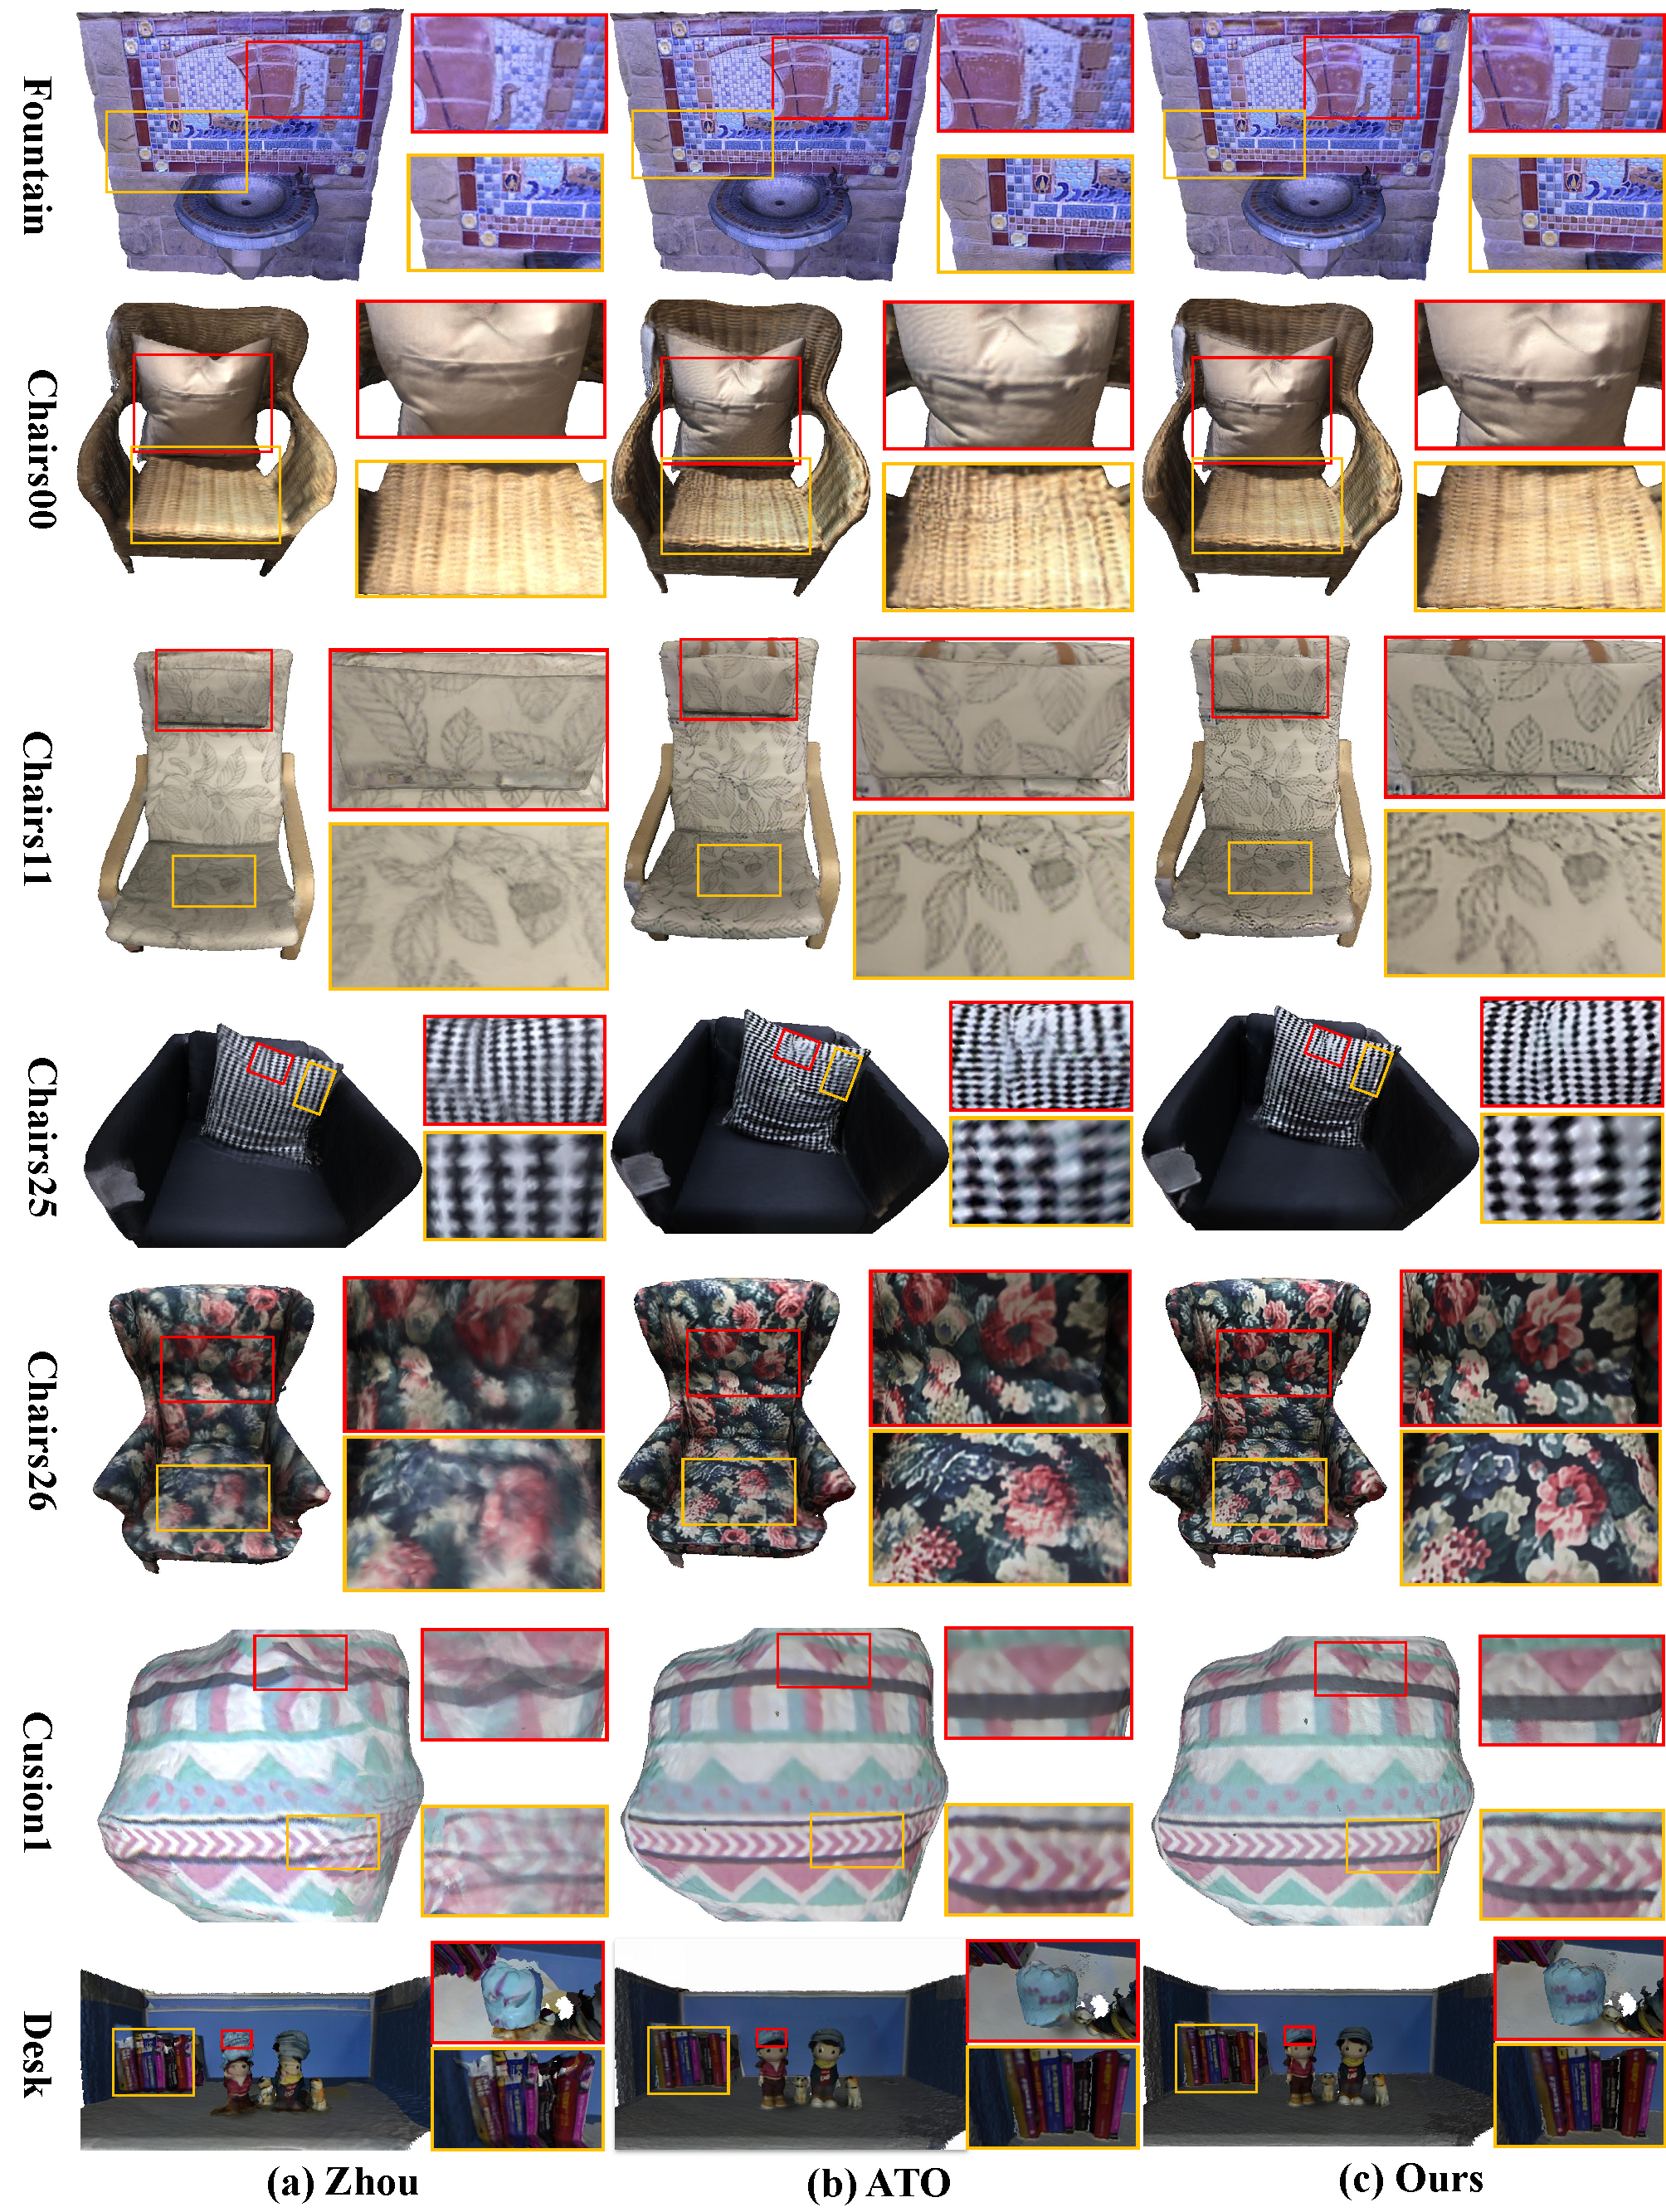
\includegraphics[width=1\linewidth]{pic/work1/visual.pdf}

\bicaption{公共数据集上不同方法的定性比较}{Qualitative comparison of different methods on public datasets}
\label{fig:ex1_1}
\end{figure}

\subsection{公共数据集上结果与分析}
本文首先在ATO\upcite{JingweiHuang2020AdversarialTO}发布的椅子数据集上数据集上进行实验比较。如图~\ref{fig:ex1_1}第二三四行所示,可以看出本文的方法得到了最佳的视觉效果,ATO采用对抗神经网络方法合成纹理图,虽然能够容忍较小的相机误差和几何误差,但是在局部地方仍然有模糊现象。例如,在$\emph{Chairs00}$ 场景下(图第一行)红色框所标注的枕头细节。本文方法与Zhou在枕头表面纹理更加平滑,不会含有噪声。在$\emph{Chairs11}$场景下,本文方法比起Zhou与ATO更加凸显椅子树叶图案的细节,如第三行红色框所展示内容。单纯的对抗生成大体上能合成貌似真实的结果,但是在相机位姿误差影响下干扰了神经网络合成图像细节的能力,这一点在纹理更加丰富的$\emph{Chairs26}$场景下更加明显。从图中橙色和红色框标注的内容上可以看出,虽然ATO纹理合成结果相比于Zhou显著减小了模糊程度,更加贴近真实结果。但是仍旧会存在伪影现象。从结果上看,本文成功地将纹理映射中的模糊伪影影响降至最低。如图第四行,在\emph{Chairs25}场景下,虽然ATO可以生成整体效果较好的纹理图像,但是在局部区域却出现了非常明显的模糊现象,导致原本清晰的黑色线条变得杂乱不清。Zhou采用顶点颜色融合方法生成纹理,当某些顶点投影位置错误时会影响加权结果导致纹理模糊,在纹理较为单一场景如$\emph{Chairs00}$与$\emph{Chair11}$下问题并不明显,但是在图案比较明显的$\emph{Chairs26}$场景下,瑕疵十分明显。例如,该场景下橙色框所展示的花瓣,图片颜色上没有区分度,局部细节存在模糊现象。本文也在Zhou发布的数据集$\emph{Scene3d}$,其中最具代表性的$\emph{Fountain}$场景下进行对比,相比于$\emph{Chairs}$数据集下的场景,该场景的视角非常稀疏,对依赖于大量数据训练的ATO与本文方法带来新的挑战。从最终结果看本文的纹理映射结果整体效果最好,无论是恢复瓷砖表面的细节(图片红色框展示)还是生成墙壁上的字体(图片橙色框展示)方面,更符合真实场景。而Zhou与ATO纹理映射结果要么存在模糊伪影,要么缺乏纹理细节。由于本文先矫正了相机位姿,为模型提供了更正确的纹理映射,又采用对抗生成方法增强纹理高频细节,所以无论从整体还是局部更符合真实场景。\par

为了证明本文在微小模型下,复杂场景下也能恢复出高保真的外观模型。本文采用Fu等人\upcite{fu2018texture}发布的数据集上进行评估。该数据集用Kinect一代相机拍摄的数据集,它获得的深度图和彩色图的分辨率较低 (640 $\times$ 480),更容易受到运动模糊,相机抖动的影响。而且获得的彩色图像中物体几何特征和色彩细节并不明显。同时该数据集上存在阴影、光照等其它噪声,相机位姿相比于$\emph{Chairs}$,$\emph{Fountain}$存在更多噪声。从图中后三行所示,Zhou只能保证场景下整体效果,但是局部细节普遍存在瑕疵。一方面源于重建模型不精确,经过中点细分又加剧了几何误差的影响。另一方面,Zhou用高斯牛顿矫正相机位姿,非刚性优化矫正内参。相比于Adam优化器\upcite{kingma2014adam}优化时梯度下降更易陷入局部最小值,残差项减小的更慢,影响了优化效果。如图$\emph{Cusion1}$场景中的黑色线条存在重影现象;$\emph{Desk}$场景下左边人物帽子未能正确产生纹理映射效果。ATO在三个场景下能生成正确纹理映射结果,但是某些细节处的伪影未能完全根除。例如,在$\emph{Bolster1}$橙色框所示图案,$\emph{Desk}$场景下人物帽子上的字体细节,人物旁边书籍名称等。本文方法相比于ATO与Zhou无论是整体视觉效果还是局部细节均展示了本文方法的优越性。\par

最后本文采用定量分析法,对整个纹理模型渲染的图像用上述介绍的评估指标进行定量分析,结果如表~\ref{tab:evluation_ex2}所示。其中G2TeX包含$\emph{Bloster1}$、$\emph{Cusion1}$、$\emph{Desk}$三个场景,$\emph{Scene3d}$包含$\emph{Fountain}$一个场景,$\emph{Chairs}$包含$\emph{Chairs00}$、$\emph{Chairs11}$、$\emph{Chairs26}$三个场景。以上所有指标均为所有场景下,不同视角渲染图片得到的度量平均值。从结果上看,本文的指标高于两者,说明纹理优化中相机位姿矫正的必要性。

\begin{table}[ht]
\bicaption{公共数据集上不同方法的定量比较}{Quantitative comparison of different methods on public datasets}
\renewcommand{\arraystretch}{1.3}

\label{tab:evluation_ex2}
	\centering
    \scalebox{0.9}[1]{
		\begin{tabular}{lcccccccccc}
            \hline
			{Datasets} & \multicolumn{3}{c}{G2Tex (3 models)}  &\multicolumn{3}{c}{Scene3d (1 models)} & \multicolumn{3}{c}{Chairs (3 models)}\\
			{} & PSNR$\uparrow$ & SSIM$\uparrow$ & Perceptual$\downarrow$ & PSNR$\uparrow$  & SSIM$\uparrow$ & Perceptual$\downarrow$ & PSNR$\uparrow$ & SSIM$\uparrow$ & Perceptual$\downarrow$ \\
			\hline
			zhou & 22.758 & 0.920 & 0.070 & 21.684 & 0.649 & 0.276 & 17.637 & 0.583 & 0.287 \\
			ATO & 23.734 & 0.941 & 0.058 & 25.463 & 0.770 & 0.269 & 21.235 & 0.680 & 0.250 \\
			Ours & \textbf{25.185} & \textbf{0.949} & \textbf{0.042} & \textbf{26.716} & \textbf{0.793} & \textbf{0.251} & \textbf{21.462} & \textbf{0.696} & \textbf{0.247} \\
            \hline
		\end{tabular}
		}
	\normalsize
\end{table}

%%
% 分别研究损失函数、仅深度图、仅彩色图。分别研究没有优化相机位姿、没有对抗生成网络情况,并添加随机噪声结果
%
\subsection{消融实验}
\begin{figure*}[ht]
\centering
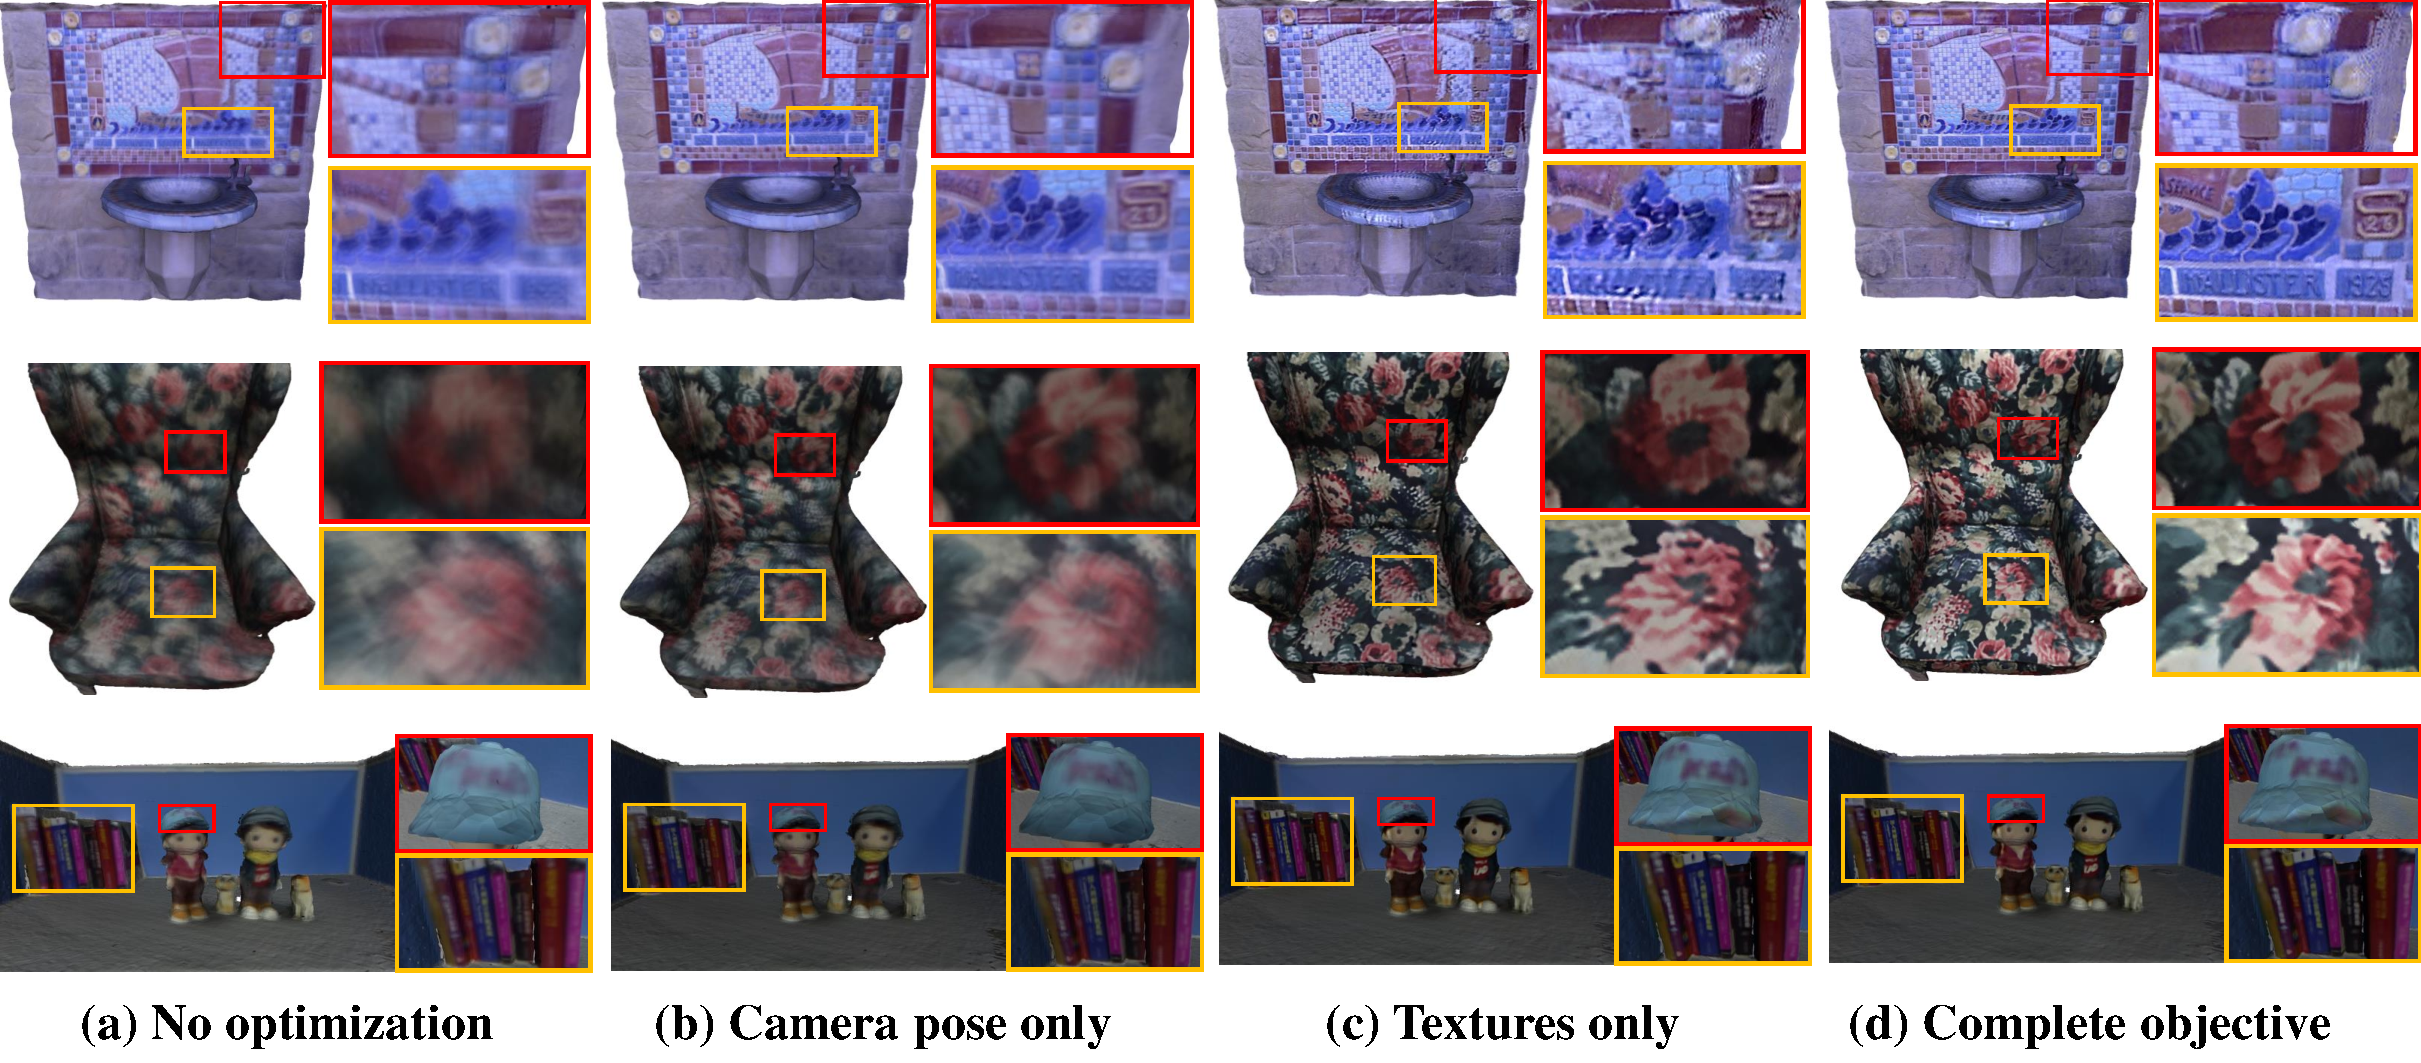
\includegraphics[width=1\linewidth]{pic/work1/final.pdf}
\bicaption{消融实验中纹理渲染结果定性比较}{Qualitative comparison of texture rendered results in ablation study}
\label{fig:ex1_2}
\end{figure*}
在这个部分,本文将研究方法中各个部分的有效性。为了更有说服力,本文选择纹理更加丰富,视觉效果强烈的$\emph{Fountain}$、$\emph{Chairs26}$、$\emph{Desk}$场景。本文分别在只矫正相机位姿,只使用对抗生成网络以及联合优化情况下展示定性结果比较。\par
如图~\ref{fig:ex1_2}所示,本文首先展示了使用图像反向投影至几何模型上生成的初始纹理映射模型(如图第一列)。在没有任何优化的情况下,视觉效果非常模糊。如图第二列所示,若没有矫正相机位姿,则渲染图片和真实图片会出现错位现象。仅仅使用可微分渲染矫正相机位姿,可以减少纹理模糊的程度,但是无法增强图像亮度、对比度等纹理细节。没有对抗生成网络时,无论是纹理细节还是整体视觉效果相比于最终结果明显下降。仅使用对抗生成网络,则可以显著提升纹理清晰度和保真度,但是存在和ATO一样的方法缺陷。本文通过矫正相机位姿,为对抗生成网络合成纹理图片寻找正确的优化方向。本文在定量评估表~\ref{tab:ablation1}中也得出了相同的结论。\par
\begin{table}[h]
\renewcommand{\arraystretch}{1.3}
\bicaption{消融实验中纹理渲染结果定量比较}{Quantitative comparison of texture rendered results in ablation study}
\label{tab:ablation1}
	\centering
%    \scalebox{0.80}{
		\begin{tabular}{lcccc}
			\hline
			{Methods} & \tabincell{c}{No pose \\ correction} &\tabincell{c}{No adversarial \\ loss} & \tabincell{c}{Complete \\ method} \\
			\hline
			PSNR$\uparrow$ & 18.515 & 24.763 & \textbf{25.330}\\
			SSIM$\uparrow$ & 0.710  & 0.764 & \textbf{0.764}\\
			Perceptual$\downarrow$ & 0.094  & 0.043 & \textbf{0.043}\\
			\hline
		\end{tabular}
%	}
%	\normalsize
\end{table}


\subsection{算法局限性}
本文的优化算法虽然已经取得了一定的成效但是仍旧有以下不足的地方。
\begin{enumerate}[label=(\arabic*),leftmargin=\parindent,align=left,labelwidth=\parindent,labelsep=0pt]
\item 无法自定义纹理坐标。本文使用\emph{obj}格式保存三维模型,需要额外存储纹理坐标以表示几何与纹理图像(UV纹理)的映射关系。\emph{ply}存储格式转为\emph{obj}格式时需要额外生成纹理坐标,但本文算法不包含纹理坐标产生流程,限制了算法通用性。
\item 需要更多的数据。本文主要使用基于深度学习的方法更新相机位姿和纹理图像,因此需要大量的训练数据来进行模型的更新。相比传统方法只需要覆盖 $360^{\circ} $ 的图像,本文需要更多的数据来获得最佳效果。在使用较小的数据集上,本文的优化效果可能会受限制,这限制了本文在小场景下的应用。
\item 在某些场景下,几何模型可能存在许多误差,即使优化纹理图像也无法保证其正确的映射关系。特别是在几何模型存在孔洞和非流形拓扑结构的情况下,这一现象将更加常见。
\end{enumerate}





\section{本章小结}

针对基于RGB-D三维重建产生的模糊纹理问题,本文提出了针对RGB-D三维重建模型的相机位姿矫正与纹理重合成结合的纹理优化算法。首先,本文输入三维重建的模型与采集得到的图片序列及其对应视角的相机位姿参数,用可微分渲染方法渲染纹理至图像,并使用重投影误差产生梯度更新相机投影矩阵;然后,用对抗生成网络重新合成新的纹理图像以适配重建模型;最后,输出一个完整且全局一致的纹理模型。实验结果表明本文的算法在大场景、小场景、在含有丰富纹理细节和含有弱纹理场景下,都能恢复出高保真的纹理,也证明了本文算法的高通用性和强鲁棒性。



